\documentclass{article}
\usepackage[utf8]{inputenc}

\title{Interrupciones}
\author{Chrsitian Gallego Chaverra}
\date{June 2020}

\usepackage{natbib}
\usepackage{graphicx}

\begin{document}

\maketitle

\section{Introducción}
Una interrupción es un mecanismo que permite ejecutar un bloque de instrucciones interrumpiendo la ejecución de un programa, y luego restablecer la ejecución del mismo sin afectarlo directamente. De este modo un programa puede ser interrumpido temporalmente para atender alguna necesidad urgente del computador y luego continuar su ejecución como si nada hubiera pasado.
Generalmente se aplica para realizar tareas elementales asincrónicas en el computador tales como responder al teclado, escribir en la pantalla, leer y escribir archivos. Un ejemplo de esta operación es la conocida Ctrl-Alt-Supr: En Windows tiene el efecto de que aparece en pantalla una lista de los procesos y ventanas en ejecución en el computador. En cambio, en el Sistema Operativo DOS cuando el usuario presiona simultáneamente dichas teclas el computador procede a reinicializarse, aunque pueda estar ocupado ejecutando un programa en ese instante. Ya sea en el sistema Windows o en DOS, el computador no está constantemente monitoreando el teclado para ver si el usuario ha solicitado un Ctrl-Alt-Supr, ya que en ese caso consumiría mucho tiempo de proceso en ello y por ende la capacidad de proceso se vería significativamente afectada. La solución empleada es una interrupción.
Luego cada vez que el usuario presiona una tecla, la CPU es advertida a través de una señal especial de interrupción. Cuando la CPU advierte/recibe una señal de interrupción suspende temporalmente el proceso actual almacenando en memoria RAM un bloque con toda la información necesaria para restablecer posteriormente la ejecución del programa si es que procede. Enseguida la CPU determina qué elemento ha solicitado la interrupción y para cada caso existe un bloque de instrucciones que realiza la tarea correspondiente que es ejecutada a continuación. Terminada la ejecución se restablece el programa original en el mismo punto en que fue interrumpido usando para ello la información almacenada previamente. \cite{InterSos}

\section{Tipos de Interrupciones}
Existen tres tipos de interrupciones:
\maketitle{Interrupciones internas de hardware}
Las interrupciones internas son generadas por ciertos eventos que surgen durante la ejecución de un programa.
Este tipo de interrupciones son manejadas en su totalidad por el hardware y no es posible modificarlas.
Un ejemplo claro de este tipo de interrupciones es la que actualiza el contador del reloj interno de la computadora, el hardware hace el llamado a esta interrupción varias veces durante un segundo para mantener la hora actualizada.
\maketitle{Interrupciones externas de hardware}
Las interrupciones externas las generan los dispositivos periféricos, como pueden ser: teclado, impresoras, tarjetas de comunicaciones, etc. También son generadas por los coprocesadores.
No es posible desactivar a las interrupciones externas.
Estas interrupciones no son enviadas directamente a la CPU, sino que se mandan a un circuito integrado cuya función es exclusivamente manejar este tipo de interrupciones. El circuito, llamado PIC 8259A, si es controlado por la CPU utilizando para tal control una serie de vías de comunicación llamadas puertos.

\begin{figure}[h]
\centering
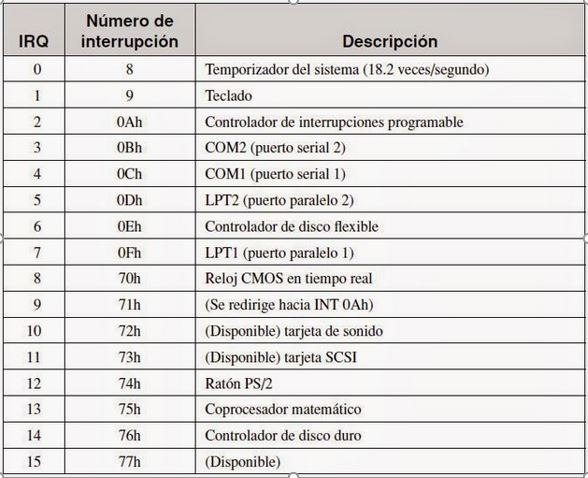
\includegraphics[scale=0.7]{interrupciones}
\caption{Interrupciones de hardware \cite{interHS}}
\label{fig:interrupciones}
\end{figure}

\maketitle{Interrupciones de software}
Las interrupciones de software pueden ser activadas directamente por el ensamblador invocando al número de interrupción deseada con la instrucción INT.
El uso de las interrupciones nos ayuda en la creación de programas, utilizándolas nuestros programas son más cortos, es más fácil entenderlos y usualmente tienen un mejor desempeño debido en gran parte a su menor tamaño.
Este tipo de interrupciones podemos separarlas en dos categorías: las interrupciones del sistema operativo DOS y las interrupciones del BIOS.
La diferencia entre ambas es que las interrupciones del sistema operativo son más fáciles de usar, pero también son más lentas ya que estas interrupciones hacen uso del BIOS para lograr su cometido, en cambio las interrupciones del BIOS son mucho más rápidas, pero tienen la desventaja que, como son parte del hardware son muy específicas y pueden variar dependiendo incluso de la marca del fabricante del circuito.
La elección del tipo de interrupción a utilizar dependerá únicamente de las características que le quiera dar a su programa: velocidad (utilizando las del BIOS) o portabilidad (utilizando las del DOS).

\begin{figure}[h]
\centering
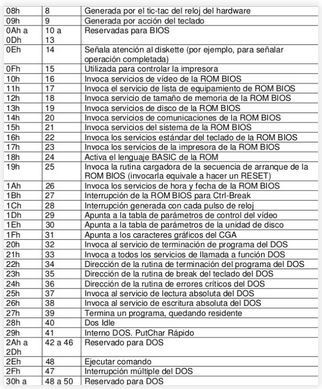
\includegraphics[scale=1.2]{interrupciones2}
\caption{Interrupciones de software \cite{interHS}}
\label{fig:interrupciones2}
\end{figure}


\section{Interrupción con Arduino}
El siguiente código empleamos el pin digital 10 para emular una onda cuadrada de intervalo 2s (1s ON y 1s OFF).
En cada interrupción actualizamos el valor de un contador. Posteriormente, en el bucle principal, comprobamos el valor del contador, y si ha sido modificado mostramos el nuevo valor.
Al ejecutar el código, veremos que en el monitor serie se imprimen números consecutivos a intervalos de dos segundos.

Para probar la interrupción en Arduino conectamos el pin 10 al 2 asociado a la interrupción 0, en la placa de Arduino.

\begin{figure}[h]
\centering
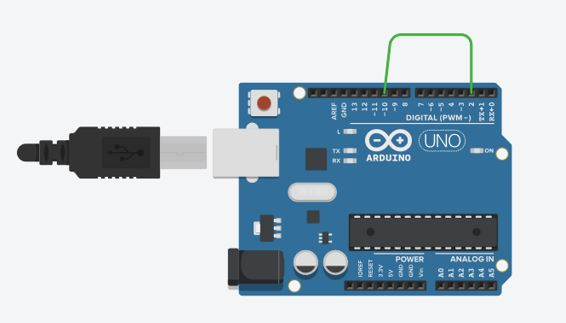
\includegraphics[scale=0.7]{interrupcionA}
\caption{Configuración de Arduino para la Interrupción}
\label{fig:interrupcionA}
\end{figure}

Luego en el código definimos los pines a utilizar y los contadores
El código y su ejecución están en el siguiente link de Tinkercad, donde se simulo la interrupción:

https://www.tinkercad.com/things/37e7SP8rarC-grand-rottis/editel 

\bibliographystyle{plain}
\bibliography{references}
\end{document}
